% IEEE conference draft. Compile on Overleaf (IEEEtran is built in) or locally with pdflatex; figures are in ./figures.
% EVERY number below is copied from measured result files in bev_rl/adaptive/results (see Section "Reproducibility").
\documentclass[conference]{IEEEtran}
\IEEEoverridecommandlockouts
\usepackage{cite}
\usepackage{amsmath,amssymb,amsfonts}
\usepackage{graphicx}
\usepackage{booktabs}
\usepackage{array}
\usepackage{textcomp}
\usepackage{xcolor}
\usepackage[hidelinks]{hyperref}
\newcommand{\ovs}{\texttt{ov\_split}}
\newcommand{\ctrl}{\texttt{ctrl\_nocaut}}
\newcommand{\cautc}{\texttt{caut\_c0}}
\newcommand{\cauta}{\texttt{caut\_auto}}
\newcommand{\todo}[1]{\textcolor{red}{[TODO: #1]}}

\begin{document}

\title{What Limits an Imitation-Learned Bird's-Eye-View Driver?\\
Expert Blind Spots, Evaluation Artefacts and Null Results\\
on Weather Conditioning in Sparse Traffic}

\author{\IEEEauthorblockN{Name 1, Name 2, Name 3, Name 4}
\IEEEauthorblockA{Department of Computer Science and Engineering, PES University, Bengaluru, India\\
Guide: Prof.\ Guide Name}}

\maketitle

\begin{abstract}
We study a compact driving policy (110{,}530 parameters) that maps a $64{\times}64$ bird's-eye-view (BEV) grid, with route and road-boundary channels, plus three scalars to steering and throttle/brake in the MetaDrive simulator at sparse traffic density (0.05). Trained with DAgger from a rule-based expert, the policy reaches 0.925 success on 200 fresh scenario seeds, against 0.745 and 0.850 for two behaviour-cloned (BC) baselines trained on five demonstrations (paired differences $+0.180$ and $+0.075$, exact McNemar $p<0.001$), and is statistically indistinguishable from its own expert. Failures concentrate in interaction scenarios (side pull-outs, oncoming drift, roundabout merges) that the expert's car-following model does not perceive. We also report what did \emph{not} work: conditioning on a caution value derived from measured detector reliability, conditioning on map-pose reliability, and PPO fine-tuning gave no gain in success. We show how a saturated validation set selected a lucky checkpoint (0.975 on 40 seeds, 0.895 on 200 fresh seeds). Weather is modelled only as simulated detector dropout calibrated from a measured YOLO retention table; the camera-to-policy pipeline is not integrated, so claims are limited to simulation.
\end{abstract}

\begin{IEEEkeywords}
imitation learning, DAgger, bird's-eye view, autonomous driving, MetaDrive, evaluation methodology, negative results
\end{IEEEkeywords}

\section{Introduction}
Camera-based driving pipelines pass perception output (detected vehicles, lane geometry) to a policy through an intermediate bird's-eye-view (BEV) representation. Two questions matter for such a policy: how well it drives when perception is good, and how it behaves when perception degrades. Much published work on adverse weather addresses perception alone; the control side is less often evaluated under controlled, paired protocols.

This paper reports a policy-side study with a deliberately narrow scope: one simulator (MetaDrive~\cite{li2022metadrive}), one traffic density (0.05), one small network. Our contributions are modest and stated precisely:
\begin{enumerate}
\item A DAgger-trained BEV policy that significantly outperforms two behaviour-cloned baselines on 200 fresh seeds and ties its privileged expert (Sec.~\ref{sec:headline}).
\item A failure analysis tying residual failures to interaction scenarios that the expert's car-following model cannot see, and a rule-based safety layer that raises the expert itself from 0.885 to 0.950 (Sec.~\ref{sec:failures}).
\item An evaluation case study: a validation set that saturates at 1.0 selects the untrained round-0 checkpoint, producing an apparent 0.975 that falls to 0.895 on fresh seeds (Sec.~\ref{sec:artefact}).
\item Controlled null results: caution conditioning, pose-reliability conditioning, and PPO fine-tuning did not improve success; we analyse why the experiments were under-powered (Secs.~\ref{sec:weather}, \ref{sec:caution}, \ref{sec:ppo}).
\end{enumerate}
We do not claim weather adaptation, energy optimisation, or end-to-end camera robustness.

\section{Related Work}
\textbf{Privileged experts and imitation.} Behaviour cloning compounds errors off the expert's state distribution; DAgger~\cite{ross2011dagger} queries the expert on the learner's own visited states. Learning by Cheating~\cite{chen2019lbc} trains a perception-limited student from a privileged teacher, and Roach~\cite{zhang2021roach} distils an RL expert into an end-to-end agent using a rendered BEV with route and lane channels plus a separate ego-measurement vector. Our input design follows this BEV-plus-vector pattern but differs in the vector contents (Sec.~\ref{sec:method}); Roach does not feed lateral offset or heading error, so our split is a design choice that should be ablated rather than assumed. ChauffeurNet~\cite{bansal2019chauffeurnet} showed that plain cloning is insufficient for complex driving.

\textbf{Causal confusion.} Cloned policies can degrade when given more input information~\cite{dehaan2019causal}; this is consistent with our scalar ablation, in which removing some inputs improved a plain MLP clone.

\textbf{Simulator and expert.} MetaDrive~\cite{li2022metadrive} provides procedural maps and traffic; its stock expert is the Intelligent Driver Model (IDM)~\cite{treiber2000idm}, which reacts only to the vehicle ahead in its lane.

\section{Problem Setting and Environment}
\textbf{Task.} The ego vehicle drives a route to a destination at MetaDrive \texttt{traffic\_density} 0.05 (sparse background traffic) with a 10\,Hz control step and an 800-step horizon at test time (600 in training). The action is $a=[\text{steer},\text{throttle/brake}]\in[-1,1]^2$. An episode ends in \emph{success} (arrival), \emph{crash}, \emph{off-road}, or \emph{timeout}.

\textbf{Energy.} We report an energy proxy (Wh/km) from positive traction work; it is a model, not a measurement.

\textbf{Seed protocol.} Scenario seeds define map and traffic. Blocks: 2000--2999 training; 3100--3109 validation/checkpoint selection; 1010--1049 ($n{=}40$) confirmation; 5000--5199 ($n{=}200$) \emph{final}, never used for any selection. All models are evaluated on identical seeds so that paired tests are valid.

\textbf{Statistics.} 95\% Wilson intervals~\cite{wilson1927}; paired differences with exact McNemar tests~\cite{mcnemar1947} and paired bootstrap intervals (10{,}000 resamples).

\section{Method}\label{sec:method}
\subsection{Inputs}
\textbf{BEV.} A $64{\times}64$ grid covering $\pm10$\,m laterally and $+17.5/-2.5$\,m longitudinally (0.3125\,m cells); values: unknown $-1$, free $0$, ego $\approx0.9$, vehicle $1.0$. The grid builder is the team's perception module and is used unmodified. The route (0.5) and road boundary (0.8) channels that the specification reserves are not drawn by that builder; we fill them from the simulator's lane geometry (a stand-in for a map and localisation stack).

\textbf{Scalars.} Speed, route progress, lateral offset, heading error, curvature, distance-to-goal, z-scored per checkpoint. Our main model (\ovs) keeps only speed, route progress and distance-to-goal, relying on the overlay for geometry.

\subsection{Network}
A conv encoder (1$\to$32, $5{\times}5$, stride 2; 32$\to$64 and 64$\to$96, $3{\times}3$, stride 2), global average pooling and a 128-d linear layer; a scalar MLP (6$\to$64$\to$32); and a head (160$\to$128$\to$2, tanh). Total 110{,}530 parameters. An optional 1-D condition input passes through Linear(1$\to$16)+ReLU and is concatenated into the head (112{,}610 parameters). The network is inherited from the project's baseline code; we did not tune its size. The condition input is read by the learned head; no rule modifies the action after the network.

\subsection{Experts}
\textbf{Stock IDM}: lane keeping plus same-lane car following. \textbf{Safety-layer expert}: IDM with lane change off plus a constant-velocity time-to-collision (TTC) check over a 3\,s horizon (hard brake below 1.3\,s TTC, soft limit below 2.4\,s). It is rule-based, uses simulator ground truth, and serves as a reference expert, not a learned model.

\subsection{Training}
DAgger rounds $r=0,1,\dots$: the student drives with probability $1-0.5^r$ (otherwise the expert acts), the expert labels every visited state, and the network is retrained on the aggregate (MSE, Adam, lr $10^{-3}$, batch 128, action noise $\sigma=0.1$). The selected checkpoint maximises validation success (ties to the earlier round).

\subsection{Compared models}
\textbf{Repo BC (sparse)} and \textbf{Repo BC (clear)}: the project's baseline checkpoints, behaviour-cloned from five IDM demonstrations (with and without traffic), GitHub BEV (no overlay), all six scalars. \textbf{\ovs}: overlay BEV, three scalars, stock-IDM DAgger. \textbf{\ctrl}: same recipe with the condition input fixed at 0, trained with detector dropout in the student's view; the selected checkpoint is round~0 (plain BC). \textbf{\cautc{} / \cauta}: one network trained with a caution-aware expert and evaluated with $c{=}0$ or $c{=}c_\text{auto}$.

\section{Weather as Detector Dropout}\label{sec:weatherdef}
MetaDrive has no weather. We obtained a \emph{retention} measurement from the team's perception stack: MetaDrive renders clean camera frames, the team's image-weather augmentation degrades them, and YOLOv8~\cite{ultralytics} runs on both. Retention is the ratio of detections under weather to detections on the clean paired frame (20 scenes, 3 placed vehicles, 2 augmentation draws). The measured values are fog~1.0: 0.267 [0.169, 0.377]; rain~0.6: 0.158 [0.097, 0.230]; rain~1.0: 0.040 [0.010, 0.081]; values above 1 are capped. In the policy simulation each vehicle is removed from the BEV independently with probability $1-\text{keep}$ at every step. This is a \emph{proxy}: retention is a count ratio (no ground-truth scoring), real misses are range-dependent and temporally correlated, and the measurement is small. Caution is $c=1-\text{keep}$ (0, 0.73, 0.84, 0.96 for clear, fog~1.0, rain~0.6, rain~1.0), a design rule rather than a derived quantity; the caution-aware expert uses $30(1-c/3)$\,km/h and a $10+15c$\,m gap.

\section{Results}
\subsection{Fresh-seed headline ($n{=}200$, clear)}\label{sec:headline}
\begin{table}[t]
\caption{Clear weather, density 0.05, 200 fresh seeds (5000--5199).}
\label{tab:n200}
\centering\small
\setlength{\tabcolsep}{3pt}
\begin{tabular}{lcccccc}
\toprule
Policy & Success [95\% CI] & Crash & Off & Wh/km & Route\\
\midrule
Safety-layer expert$^\dagger$ & .950 [.910,.973] & .010 & .040 & 101.3 & .968\\
\ovs & \textbf{.925} [.880,.954] & .060 & .010 & 96.2 & .939\\
\ctrl & .895 [.845,.930] & .105 & .000 & 80.4 & .932\\
Stock IDM$^\dagger$ & .885 [.833,.922] & .080 & .035 & 97.9 & .933\\
Repo BC (clear) & .850 [.794,.893] & .125 & .025 & 85.9 & .918\\
Repo BC (sparse) & .745 [.680,.800] & .120 & .135 & 90.7 & .883\\
\bottomrule
\end{tabular}\\[2pt]
{\footnotesize $^\dagger$ rule-based reference experts (simulator ground truth), not learned models.}
\end{table}
\begin{table}[t]
\caption{Paired success differences on identical seeds ($n{=}200$).}
\label{tab:paired}
\centering\small
\setlength{\tabcolsep}{3pt}
\begin{tabular}{lccc}
\toprule
Comparison (A$-$B) & Diff [95\% CI] & A-only/B-only & McNemar $p$\\
\midrule
\ovs $-$ Repo BC (sparse) & +.180 [+.125,+.240] & 38/2 & $<$.0001\\
\ovs $-$ Repo BC (clear) & +.075 [+.035,+.120] & 17/2 & .0007\\
\ovs $-$ stock IDM & +.040 [.000,+.080] & 12/4 & .077\\
\ovs $-$ safety-layer expert & $-$.025 [$-$.075,+.020] & 9/14 & .40\\
\ovs $-$ \ctrl & +.030 [$-$.005,+.065] & 10/4 & .18\\
Safety-layer $-$ stock IDM & +.065 [+.030,+.105] & 15/2 & .0023\\
\bottomrule
\end{tabular}
\end{table}
\ovs{} outperforms both behaviour-cloned baselines significantly and is indistinguishable from the safety-layer expert and, marginally, from the stock IDM it was trained on (Tables~\ref{tab:n200}, \ref{tab:paired}). \emph{Attribution caveat:} the baselines use five demonstrations while \ovs{} uses about 73\,k aggregated DAgger samples, and three design factors differ (data, algorithm, input design), so the comparison establishes that the whole system is better, not which factor is responsible. An isolating ablation at $n{=}200$ is left to future work; the earlier DAgger model without overlay (0.875 at $n{=}40$) is not significantly different from \ovs{} (0.925).

\subsection{Failure analysis}\label{sec:failures}
\ovs{} fails 15 of 200 seeds (12 crashes, 2 off-road, 1 timeout). Fourteen of these are seeds the safety-layer expert completes, so they are in principle avoidable (headroom $\le 0.07$); conversely \ovs{} succeeds on 9 of the expert's 10 failures. Tracing seeds 1019, 1039 and 1040 shows a pull-out from a side lane, an oncoming vehicle drifting into the ego lane while the ego is centred, and a roundabout merge. The stock IDM reacts only to the vehicle ahead in its own lane, so it cannot respond to these; students trained from it inherit the gap. Adding the TTC layer improves the expert itself from 0.885 to 0.950 ($p=0.0023$). We do not claim the causal link from expert blind spot to student failure is proven; the seed-level overlap is consistent with it.

\subsection{An evaluation artefact: 0.975 $\to$ 0.895}\label{sec:artefact}
\begin{figure}[t]
\centering
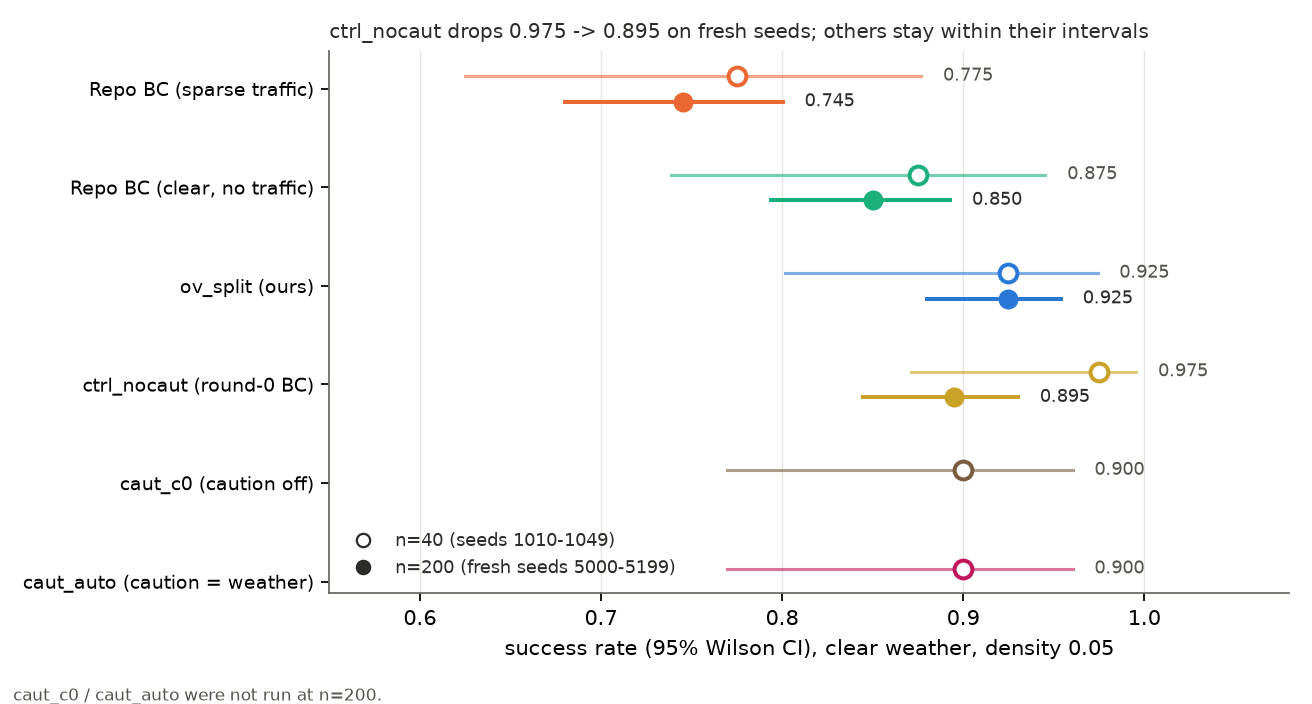
\includegraphics[width=\columnwidth]{figures/n40_fig6_n40_vs_n200_clear.png}
\caption{Clear-weather success at $n{=}40$ (open) and $n{=}200$ fresh seeds (filled). \ctrl{} drops from 0.975 to 0.895; other models stay within their intervals.}
\label{fig:rep}
\end{figure}
On the 40-seed confirmation block \ctrl{} scored 39/40 (0.975) in every weather, above \ovs{} (0.925). The checkpoint is DAgger round~0 (plain BC from the expert, 16{,}835 samples): validation success was 1.0 in every round, so the tie-break kept the earliest round. The 40-seed block had also been inspected while choosing it, and 39/40 versus 37/40 is a two-episode gap with overlapping intervals. On 200 fresh seeds it scores 0.895 (Fig.~\ref{fig:rep}). Later rounds did not help (round~2: 0.80, round~5: 0.925 on 40 seeds). The lesson is methodological: validation must not saturate, and selection and test seeds must be disjoint.

\subsection{Weather as detector dropout ($n{=}40$ per cell)}\label{sec:weather}
\begin{table}[t]
\caption{Success under simulated detector dropout, density 0.05, seeds 1010--1049 ($n{=}40$, intervals $\approx\pm0.12$). $^\ast$selection-biased (Sec.~\ref{sec:artefact}).}
\label{tab:weather}
\centering\small
\setlength{\tabcolsep}{3pt}
\begin{tabular}{lcccc}
\toprule
Policy & Clear & Fog 1.0 & Rain 0.6 & Rain 1.0\\
keep-prob & 1.00 & 0.27 & 0.16 & 0.04\\
\midrule
Repo BC (sparse) & .775 & .800 & .800 & .800\\
Repo BC (clear) & .875 & .875 & .875 & .875\\
\ovs & .925 & .925 & .925 & .950\\
\ctrl$^\ast$ & .975 & .975 & .975 & .975\\
\cautc & .900 & .900 & .900 & .900\\
\cauta & .900 & .925 & .900 & .850\\
\bottomrule
\end{tabular}
\end{table}
Success is flat for every policy except \cauta{} (Table~\ref{tab:weather}). For \ovs{} the failed seeds are identical in clear, fog and rain~0.6 (1019, 1039, 1040) and rain~1.0 recovers one, i.e.\ failures follow the scenario, not the weather. We interpret this as \emph{insensitivity} to our dropout model, not robustness: at density 0.05 there are few vehicles, the policies rely mainly on the map overlay and scalars, and no reference policy degraded. A robustness claim would need a regime in which a reference policy loses success first. A paired comparison with the sparse-traffic baseline at $n{=}40$ is significant only in clear weather ($+0.150$, $p=0.031$).

\subsection{Caution conditioning: no success benefit}\label{sec:caution}
\cauta{} is the only policy whose behaviour changes with weather: mean speed falls from 8.02 to 5.58\,m/s and energy from 84.7 to 56.1\,Wh/km as $c$ rises, crashes drop from 0.10 to 0 but timeouts rise to 0.15, and success is 0.850 in rain~1.0 (Table~\ref{tab:weather}). This reproduces the speed ($\approx$20\,km/h at $c{=}1$) that the caution-aware expert was designed to produce, so it shows the student learned the specified mapping, not that caution improves safety. Because weather did not degrade any baseline, the experiment had nothing to rescue; we treat it as uninformative on safety and informative only as an energy/time trade-off.

\subsection{Map-pose error}\label{sec:loc}
\begin{table}[t]
\caption{Success versus lateral map-pose error (heading error scaled together), clear weather, $n{=}40$ per level.}
\label{tab:loc}
\centering\small
\setlength{\tabcolsep}{3pt}
\begin{tabular}{lccccc}
\toprule
Policy & 0 & 0.25\,m & 0.5\,m & 1.0\,m & 2.0\,m\\
\midrule
Repo BC (sparse) & .775 & .600 & .550 & .225 & .150\\
DAgger, no overlay & .875 & .750 & .500 & .275 & .300\\
\ovs & .925 & .900 & .900 & .700 & .275\\
\bottomrule
\end{tabular}
\end{table}
\ovs{} keeps $\ge0.90$ up to 0.5\,m and beats the sparse baseline by $+0.30$, $+0.35$, $+0.475$ at 0.25, 0.5, 1.0\,m ($p=0.004$, $0.0005$, $<0.0001$); at 2\,m all policies collapse (Table~\ref{tab:loc}). \emph{Caveat:} the perturbation is a shift of the overlay for overlay models but an offset on the lateral/heading scalars for the baseline (which has no overlay), so the comparison is not like-for-like. Conditioning on the injected error level did not help; a second noisy lateral/heading cue rescued large errors, but the benefit came from the cue, not from conditioning, and with a noisy second cue the conditioned model was worse.

\subsection{PPO fine-tuning: no gain, and why}\label{sec:ppo}
Five PPO reward variants (150\,k steps, lr $5{\times}10^{-5}$, started from \ovs) stayed within noise of the starting score (0.35 on a 40-episode mixed-traffic validation set, s.e.\ $\approx0.075$; end scores 0.325--0.400). We attribute this to: little headroom ($\le0.07$ at density 0.05), a budget of about 250 episodes (5{,}900 gradient steps), a reward with no headway term, and checkpoint selection as a maximum over noisy scores. At $n{=}200$ the smallest paired gain detectable with 80\% power is about 0.067 (about 0.034 at $n{=}800$), so a modest true gain could not be detected. This is an uninformative null, not evidence that RL cannot help.

\subsection{An energy observation}
\ctrl{} uses $15.8$\,Wh/km less than \ovs{} on the same 200 seeds (paired 95\% CI $[-19.4,-12.7]$), at slightly higher speed ($+0.12$\,m/s); restricted to the 175 seeds both complete the difference is $-13.1$ [$-15.6,-10.9$]. Its success deficit ($-0.030$) is not significant. We have not identified the cause; this is an observation from a single training seed, not an energy-optimisation result.

\section{Threats to Validity and Limitations}
\begin{itemize}
\item \textbf{No integrated camera pipeline.} The policy never saw an image; it consumes simulator-derived BEVs with synthetic vehicle dropout.
\item \textbf{Weather proxy.} Count-ratio retention, small sample, independent per-step dropout; no weather physics in MetaDrive.
\item \textbf{Map from the simulator.} Route/boundary channels come from the simulator's lane geometry.
\item \textbf{Single training seed} per configuration; across-seed variance is unmeasured.
\item \textbf{Confounded baselines} (data, algorithm, inputs) and $n{=}40$ weather cells with $\pm0.12$ intervals.
\item \textbf{Simulation only}, one scenario family.
\end{itemize}

\section{Conclusion and Future Work}
A compact DAgger-trained BEV policy beats few-demonstration cloning and ties its expert in sparse MetaDrive traffic; residual failures concentrate where the expert is blind; and several plausible additions (caution, pose conditioning, PPO) gave no measured success gain, partly because the experiments could not have shown one. Future work: (i) evaluate the student trained from the safety-layer expert, which is trained but not yet reported here, to test whether a better expert yields a better student; (ii) an isolating ablation of overlay, scalar split and DAgger at $n\ge200$ with several training seeds; (iii) a regime where degradation demonstrably hurts a reference (interaction-critical scenarios, range-dependent and temporally correlated misses); (iv) closed-loop camera-in-the-loop validation of the dropout proxy.

\section*{Reproducibility}
Seeds, scripts and result files are in the project repository; tables here are generated by \texttt{paper/make\_*} scripts from \texttt{bev\_rl/adaptive/results}. \todo{add repository link and commit hash before submission}

\begin{thebibliography}{99}
\bibitem{li2022metadrive} Q.~Li, Z.~Peng, L.~Feng, Q.~Zhang, Z.~Xue, and B.~Zhou, ``MetaDrive: Composing diverse driving scenarios for generalizable reinforcement learning,'' \emph{IEEE Trans.\ Pattern Anal.\ Mach.\ Intell.}, vol.~45, no.~3, pp.~3461--3475, 2023.
\bibitem{ross2011dagger} S.~Ross, G.~J.~Gordon, and J.~A.~Bagnell, ``A reduction of imitation learning and structured prediction to no-regret online learning,'' in \emph{Proc.\ AISTATS}, 2011, pp.~627--635.
\bibitem{chen2019lbc} D.~Chen, B.~Zhou, V.~Koltun, and P.~Kr\"ahenb\"uhl, ``Learning by cheating,'' in \emph{Proc.\ CoRL}, 2019, pp.~66--75.
\bibitem{zhang2021roach} Z.~Zhang, A.~Liniger, D.~Dai, F.~Yu, and L.~Van~Gool, ``End-to-end urban driving by imitating a reinforcement learning coach,'' in \emph{Proc.\ ICCV}, 2021, pp.~15222--15232.
\bibitem{bansal2019chauffeurnet} M.~Bansal, A.~Krizhevsky, and A.~Ogale, ``ChauffeurNet: Learning to drive by imitating the best and synthesizing the worst,'' in \emph{Proc.\ Robotics: Science and Systems}, 2019.
\bibitem{dehaan2019causal} P.~de~Haan, D.~Jayaraman, and S.~Levine, ``Causal confusion in imitation learning,'' in \emph{Proc.\ NeurIPS}, 2019.
\bibitem{treiber2000idm} M.~Treiber, A.~Hennecke, and D.~Helbing, ``Congested traffic states in empirical observations and microscopic simulations,'' \emph{Phys.\ Rev.\ E}, vol.~62, no.~2, pp.~1805--1824, 2000.
\bibitem{wilson1927} E.~B.~Wilson, ``Probable inference, the law of succession, and statistical inference,'' \emph{J.\ Amer.\ Statist.\ Assoc.}, vol.~22, no.~158, pp.~209--212, 1927.
\bibitem{mcnemar1947} Q.~McNemar, ``Note on the sampling error of the difference between correlated proportions or percentages,'' \emph{Psychometrika}, vol.~12, no.~2, pp.~153--157, 1947.
\bibitem{ultralytics} G.~Jocher, A.~Chaurasia, and J.~Qiu, ``Ultralytics YOLOv8,'' software, 2023. [Online]. Available: https://github.com/ultralytics/ultralytics
\end{thebibliography}

\end{document}
